\chapter{General Prologue}
\section{Introduction}
Condensed matter physics is a subject about \emph{phases}. In fact, the central topics of condensed matter physics are
\begin{enumerate}
    \item to discover novel quantum state of phases;
    \item to understand the intricate phase transitions among them.
\end{enumerate}
Clearly it is sensible to talk about the transitions between phases only \emph{after} we get to know what exactly theses phases are.

The concept of phases is developing along with the growth of condensed matter physics in the past centry. There are two milestones: the concept of \emph{Landau fermi liquid} and the phenomena of \emph{spontaneous symmetry breakings}. Landau fermi liquid theory adiabatically connects the interacting electronic fluids with the non-interacting electron gas, with introduction of \emph{quasiparticles} [Landau, Abrikosov]. Quasiparticles has become the most fundenmental object to describe the weakly-interacting systems. This object is so universal that it was believed to constitute our real world at every energy scales. In the pioneering paper of Anderson \cite{anderson1972more}, the philosophy of \emph{emergence} was first proposed, as an independent declaration of condensed matter physics, wherein spontaneous symmetry breaking is explained as the fundamental mechanism for the emergent behavior of quasiparticles at different energy scales.

Spontaneous symmetry breaking is really not a new concept: it occurs everyday in our normal life. Taking water as the example, as a normal fluid it is continuously translational-invariant and isotropic, or has $\mathbb R^3\times\mathrm{O}(3)$ symmetry in the language of group theory. When cooling down below the freezing point, solid ice will be formed, leaving just discrete translation symmetry and discrete rotation symmetries.


Due to the early success in explanation of Fermi liquid \cite{landau1959theory}, He-II superfluidity \cite{landau1941theory}, and BCS superconductivity \cite{bardeen1957theory,bardeen1957microscopic}, it has been a long time for people to believe that the combined paradigm of Landau fermi liquid theory (with quasiparticles) and spontaneous symmetry breaking, tells the whole story of condensed matter theory. With the help of renormalization group (RG) analysis, people at that time even tends to believe that everything in condensed matter physics is predictable, as long as the quasiparticle properties and system symmetries are given.

However, the subsequntly discoveries of unconventional high-$T_c$ superconductivity beyong BCS theory, from cuprates \cite{bednorz1986possible}, to iron-based superconductors \cite{kamihara2006iron} and Nickel-based superconductors \cite{li2019superconductivity}, from bulk materials like YBCO [] and BiSSCO [] to thin-film materials like monolayer FeSe \cite{liu2012electronic} and twisted bilayer graphene (tBLG) \cite{cao2018correlated,cao2018unconventional}, have all declared the breakdown of quasiparticle pictures. And the discoveries of integer quantum Hall effect (IQHE) \cite{klitzing1980new} and fractional quantum Hall effect (FQHE) \cite{tsui1982two,willett1987observation}, together with the following proposals and realizations on the huge family of topological insulators (TI) \cite{bernevig2006quantum,hsieh2008topological} and topological superconductors \cite{xu2014artificial}, have all revealed the importance of \emph{topology} in condensed matter physics, which has been longly overlooked by the traditional paradigm of Landau fermi liquid thoery and spontaneous symmetry breakings. Particularly, nowadays \emph{topological orders} \cite{wen1990topological,levin2005string,chen2010local,wen2002quantum}, first proposed by Wen in understanding of the ground state degeneracy in FQHE \cite{wen1990ground}, has become the fundamental language in describing and classification of these phenomena. And the interplay between topological orders and \emph{symmetries} has been further developed into a vast framework classifying all quatum phases of matter in our universe, including \emph{symmetry-protected topological trivial states (SPT)} \cite{chen2013symmetry} and \emph{symmetry-enriched topological orders states (SET)} \cite{mesaros2013classification}.

It can be seen that the concept of phases in condensed matter physics has been highly complexified due to the interplay of symmetry, topology, and strong-correlations. In this thesis, I will focus on the study of the quantum phases of matter in two-dimensional (2D) space, particularly in the context of the \emph{twisted} 2D materials exhibiting all these complexities. The thesis is organized as follows
\begin{itemize}
    \item In the beginning, I will generally introduce the complexity brought by dimensionality (particularly 2D), symmetry and topology. I will take graphene and transition metal dichalcogenides as two typical examples of 2D materials, and discuss the complexity carried by the new tunability of twisting angles, especially on \emph{Moir\'{e} physics}.
    \item Then as the main part of the thesis, I will list three of my works on twisted 2D materials. The former two works are about 2D superconductors, where complexities of free-fermion topology, symmetries, and twistings are involved. The other recent long work is for \emph{fractional Chern insulators} (FCI), the lattice analogue of FQHE. In construction of the framework, all factors of complexity mentioned above get intertwined, including Moir\'{e} physics, strong correlations, and symmetry-enriched topological orders.
\end{itemize}

\section{Complexity from Dimensionality: 2D}
In this section, I will briefly discuss the complexity of the condensed matter systems from the perspective of dimensionality. Particularly, I will focus on the two-dimensional systems, as it is the main topic of this thesis. \textbf{[todo!]}
\begin{itemize}
    \item \textbf{Statistics in 2D: Anyons.} The most famous example exhibiting the particularity of the two-dimensional space is on the classification of elementary particles. The modern thoery explaining the statistics of elementary particles is to consider the \emph{dynamic process of braiding} \cite{laidlaw1971feynman,wu1984general}. In path-integral formalism, it is
          \begin{equation*}
              _f\langle \{\bm x_N\}|\{\bm x_N\}\rangle_i\equiv\int_{\gamma}\mathcal D\{\bm x_N\}\, e^{iS[\{\bm x_N\}]}=\sum_{[\gamma]\in\pi_1(M_N)}\chi([\gamma])\int_{\gamma\in[\gamma]}\mathcal D\{\bm x_N\}\, e^{iS[\{\bm x_N\}]}.
          \end{equation*}
          Here we sum up all paths $\gamma\in M_N$ of the configuration space $M_N$ connecting the initial/final states. We further grouped them into topologically inequivalent sectors, classified by the first homotopy class $\pi_1(M_N)$.

          Clearly $M_N\subset\mathbb R^{Nd}=\mathbb R^d\times\cdots\times\mathbb R^d$ is the subspace of the full $N$-particle configuration space. Now because we are interested in the braiding processes only, all the trivial configurations that have particles occupying the same positions $\Delta=\{(\bm x_1,\cdots,\bm x_N)|\exists i\neq j, \bm x_i=\bm x_j\}$ should be excluded. Due to the indistinguishability of $N$-particles, any mutual exchange (relabeling) of particles described by the permutation group $S_N$ should be considered as the same configuration . As a result, the configuration space $M_N=(\mathbb R^{Nd}\backslash \Delta)/S_N$. Depending on the spatial-dimensionality, we have the following results \cite{wu1984general}:
          \begin{itemize}
              \item In $d=1$: there is no sense to talk about braiding operations.
              \item In $d=2$: $\pi_1(M_N)=B_N\equiv\langle\sigma_1\cdots\sigma_{n-1}|\sigma_i\sigma_j=\sigma_j\sigma_i,\sigma_i \sigma_{i+1}\sigma_i=\sigma_{i+1}\sigma_i \sigma_{i+1}\rangle$ is the \emph{braid group}.
              \item In $d\geq3$: $\pi_1(M_N)=S_N\equiv\langle\sigma_1\cdots\sigma_{n-1}|\sigma_i^2=1,\sigma_i\sigma_j=\sigma_j\sigma_i,\sigma_i \sigma_{i+1}\sigma_i=\sigma_{i+1}\sigma_i \sigma_{i+1}\rangle$ is the \emph{permutation group}.
          \end{itemize}
          For one-dimension representations $\rho:\sigma_i\mapsto e^{i\theta_i}$, the presentation constraints shared by $S_N$ and $B_N$ simply tells $\theta_i=\theta_{i+1}=\theta$. Relation $\sigma_i^2=1$ in $S_N$ futher fixes $\theta=0,\pi$, or weight $\chi_\pm([\alpha])=\pm1$ as the sign of the permutations, explaining the \emph{spin-statistics theorem} or the origin of bosons/fermions in $(3+1)$-d field theory. For braid group, however, $\chi_\theta([\alpha])=e^{i\theta}$ can be chosen arbitrarily. Each abelian representation $\chi_\theta$ corresponds to one \emph{abelian anyons} \cite{wilczek1982quantum}.

          The above argument \emph{implicitly assume that the Hilbert space of a collection of particles at specified positions is one-dimensional}. If we release that assumption by considering a many-particle state with extra $\mathcal D$-degeneracy (the \emph{total quantum dimension} \cite{kitaev2006topological,levin2006detecting}) apart from the degeneracy in conventional sense such as single-particle's spin/flavor/valley/band indices, then the amplitude between the initial/final states becomes
          \begin{equation*}
              _f\langle\{\bm x_N\},n|\{\bm x_N\},n'\rangle_i=\sum_{[\gamma]\in\pi_1(M)}\chi_{nn'}([\gamma])\int_{\gamma\in[\gamma]}\mathcal D\{\bm x_N\}\, e^{iS[\{\bm x_N\}]},
          \end{equation*}
          where $\mathcal D$-dimensional non-abelian representation $\chi:\pi_1(M_N)\rightarrow\mathrm{GL}_{\mathcal D}(V)$ enters. In two-dimensional space, $\chi: B_N\rightarrow\mathrm{GL}_{\mathcal D}(V)$ gives the classification of \emph{non-abelian anyons}\footnote{The \emph{parastatistics}, named for non-abelian representation of higher dimensional space, though exits in mathematical sense, is excluded in the path integral formalism in the long proof of Ref. \cite{laidlaw1971feynman}}. Besisdes the non-abelian mutual statistics, there is another intrinsic property called the \emph{fusion rules} $\phi_a\star\phi_b=\sum_c N^c_{ab}\phi_c$ by considering the composite particle . As an appreciation of the complexity in 2D, it is enough to pause the discussion here.

    \item \textbf{Disorder in 2D: Weak Localization.} In the seminal paper by ``the gang of four'' Abrahams, Anderson, Licciardello, and Ramakrishnan in Ref. \cite{abrahams1979scaling}, a scaling theory is constructed with the strong hypothesis that the change of the conductance $G$ with the length scale $L$ depends solely on the conductance at previous length scales, and not, for example, independently on $L$ or on the strength of the disorder. The RG equation for the conductance is then a single-parameter scaling equation
          \begin{equation*}
              \dfrac{\mathrm d\ln G}{\mathrm d\ln L}=\beta(G(L)).
          \end{equation*}
          In the weak disorder limit $G\gg1$ where Ohm's law is expected to hold (or microscopically the diffusive Drude physics dominates), the conductance $G=1/R=\sigma\frac{L}{A}\sim\sigma L^{2-d}$, giving
          \begin{equation*}
              \lim_{\ln G\rightarrow\infty}\beta(G)=d-2.
          \end{equation*}
          While in the strong disorder limit $G\ll1$ where Anderson's strong-disorder perturbation thory [] holds, and the conductance should drop off exponentially with the system size $G(L)=G_0 e^{-L/\xi}$, or
          \begin{equation*}
              \lim_{\ln G\rightarrow-\infty}\beta(G)=-\frac{L}{\xi}\simeq\ln G\rightarrow-\infty.
          \end{equation*}
          Naive smooth connection of these two limit regimes tells that (see Fig. \ref{fig:scaling_of_Anderson_localization})
          \begin{itemize}
              \item In $d=1$: $\beta(G)<0$ and the system will always flow to the insulating regime.
              \item In $d=2$: marginal case.
              \item In $d=3$: there is one critical point $G_c$ above which the system will flow to the metallic regime, and below which the system will flow to the insulating regime.
          \end{itemize}
          \begin{figure}[!htp]
              \centering
              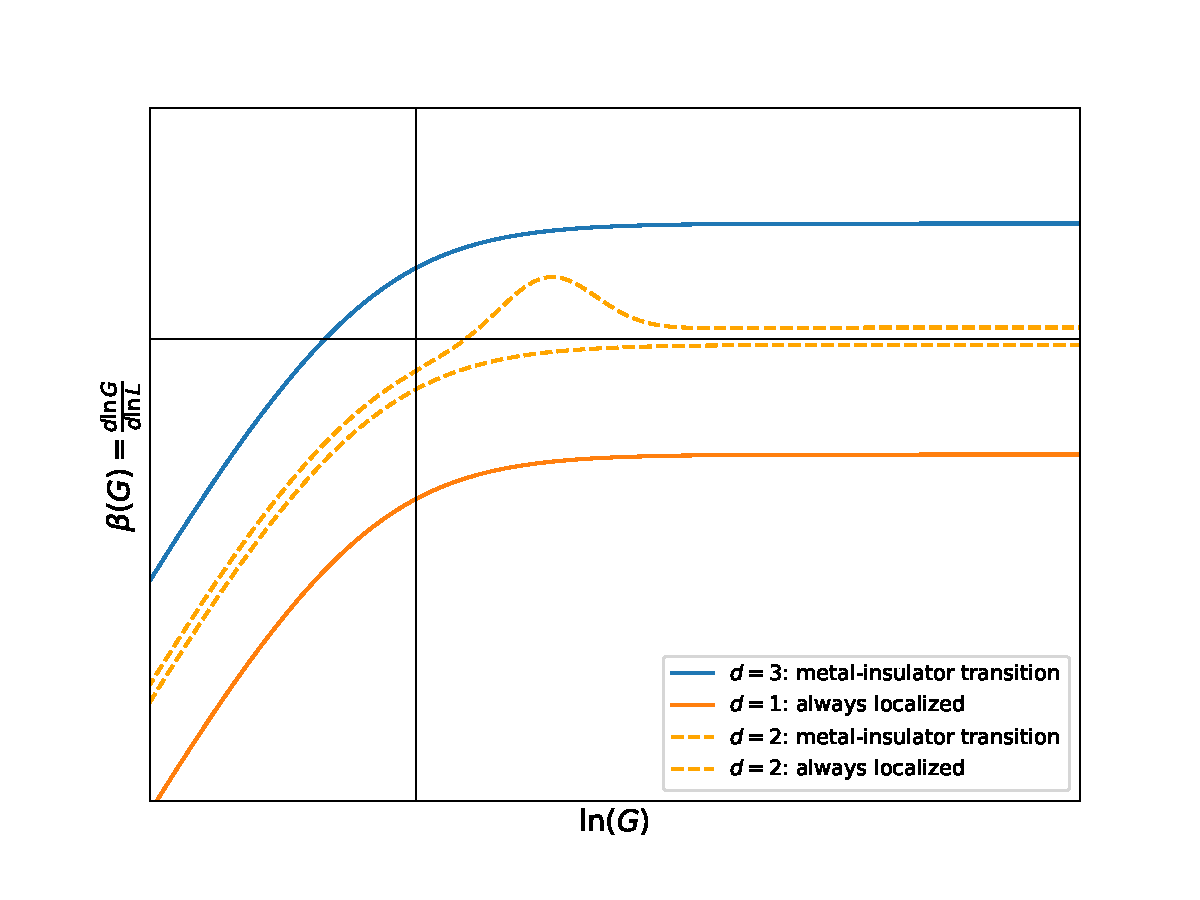
\includegraphics[width=0.7\textwidth]{figures/scaling_of_Anderson_localization.pdf}
              \caption{Schematic Plot on the RG Flow of the Conductance}
              \label{fig:scaling_of_Anderson_localization}
          \end{figure}
\end{itemize}

\section{Complexity from Symmetry and Topology}
Modern classification theory on quantum phases of matter is based on the intrinsic property of the quantum states: quantum entanglement. The concept of \emph{local unitary transformation} (LU) was proposed first in classificaltion of the matrix product states representation of the 1D gapped spin systems
\begin{equation*}
    |\Psi\rangle=\sum_{s_1,\cdots,s_N}\mathop{\mathrm{Tr}}\bigg[A_1^{s_1}A_2^{(s_2)}\cdots A_N^{(s_N)}\bigg]|s_1,s_2,\cdots,s_N\rangle,
\end{equation*}
by Chen, Gu and Wen in \cite{chen2011classification} . They quickly realize that the framework of LU can be generalized to other quantum phases in \cite{chen2010local}, resulting in the famous map:

\subsection{Free fermion Topology: Example of 10-fold Way}
The key feature of SPT state is the presence of the \emph{gapless} edge states that are protected by the symmetry. Namely we


\subsection{Symmetry Enrichment: SPT and SET}
Symmetry protected topological (SPT) order exists in gapped systems with global symmetry. The ground state of the system does not spontaneously break the symmetry, has no fractional excitation, yet cannot be smoothly connected to a product state without explicitly breaking the symmetry. The nontrivial natural of the SPT order can be manifested in two ways:
\begin{enumerate}
    \item As nontrivial edge states which must either be gapless, spontaneously break symmetry or support anomalous SF pattern (with bulk dimension $\geq3$) as long as the global symmetry is not explicitly broken.
    \item For SPT phases with unitary on-site symmetry, gauging the symmetry results in nontrivial gauge theories whose gauge fluxes have nontrivial braiding statistics.
\end{enumerate}

It was shown that a large class of SPT phases in boson/spin systems in dimension d has a one to one correspondence with equivalence classes of group cocycles $H^{d+1}(G, U (1))$ [Witten]. For unitary G, gauging the symmetry results in $d$ dimensional Dijkgraaf-Witten (DW) gauge theory characterized also by the equivalence class of cocycles []. For example, the double semion theory in 2D is a DW gauge theory of gauge group $\mathbb Z_2$ corresponding to the nontrivial element in $H^3 (\mathbb Z_2 , U(1))$. For definition of group cocycles and discussion of their relation with SPTs and gauge theories , see Refs. [].
For the discussion in this review, it suffices to know that the set of equivalence classes of group cocycles in $H^{d+1}(G, U (1))$ forms an abelian group. For $d=0$, elements in $H^1(G, U(1))$ corresponds to one dimensional representations of $G$ which have a one to one correspondence with symmetry charges of $G$. For $d=1$, elements in $H^2(G, U(1))$ corresponds to projective representations of $G$ with $U(1)$ coefficient; such projective representations are realized as degenerate edge states of one dimensional SPT phases. We collect a few simple mathematical results of $H^{d+1}(G, U (1))$, for $d\geq1$, ...


\section{Complexity from Twisting: Moir\'{e} Physics}
\subsection{2D Materials}
\subsubsection{Graphene}
Historically, there exists many arguments claiming the non-existence of 2D materials due to the instability under finite thermal fluctuations\footnote{For example, a naive (so \emph{wrong}) entropy argument goes as following: Note that 2D material has less vibration modes than 3D materials of the same particle number, the entropy contribution from these vibration modes should be smaller in 2D, so is not entropy-favored.}, and even Lev Landau made mistakes here\footnote{Landau claim the non-existence based on the experimental facts that no divergence has been observed under a disorder to order (like liquid to crystal) phase transition.}. All of these arguments are disputed by the discovery of graphene in 2004 by Geim and Novoselov \cite{novoselov2004electric}. And the realistic two-dimensional world has been opened since then.

Graphene is well-known for the appearance of Dirac points in its band structure. For the honeycomb lattice constituted of carbon atoms only, there exists sublattice (inversion) symmetry between $A,B$ sublattices. For spinless electrons, where Hamiltonian is written in such pseudospin basis as a general two-by-two matrix $H(\bm k)=\bm d(\bm k)\cdot\bm \tau$ with real vector coefficients $\bm d(\bm k)$, the inversion operator $\mathcal P$ exchanging $A,B$ sites can be represented as $P=\tau_x$. Graphene also possesses time-reversal symmetry, and for spinless electrons the time-reversal operator is simply a complex conjugate $T=K$. Therefore, the combination of inversion symmetry and time-reversal symmetry keeping the momentum unchanged: $\mathcal P\mathcal T:\bm k\mapsto\bm k$, requires the Hamiltonian to satisfy
\begin{equation*}
    \tau_x^{-1}H^*(\bm k)\tau_x=H(\bm k),
\end{equation*}
implying $d_3(\bm k)=0$ or $H(\bm k)=d_1(\bm k)\tau_x+d_2(\bm k)\tau_y$ with ALL matrix element off-diagonal. Now because both the momentum and the Hamiltonian share the same dimensionality, \emph{given one zero solution of the eigen equation $\det|\lambda I-H(\bm k)|=0$, any perturbation preserving the inversion and time-reversal symmetries, i.e., constituted of $\tau_x$ and $\tau_y$ matrices, cannot destroy such zero point}. That is the typical example of symmetry-protected Dirac points (if exists) in graphene.

To obtain the low-energy description of graphene, we can consider the spatial $C_3$ rotation symmetry at the $K$ and $K'$ points, and implement the constraint from $C_3$ rotation operations that
\begin{equation}\label{eq:C3 rotation constraint}
    C_3^{-1}H(\bm k)C_3=H(\mathcal C_3^{-1}\bm k).
\end{equation}
\noindent Precisely speaking, we can expand the general Hamiltonian around $K$ and $K'$ to the lowest linear-order
\begin{equation*}
    d_1(\bm k)=a_{10}+a_{11}k_x+a_{12}k_y,\quad d_2(\bm k)=a_{20}+a_{21}k_x+a_{22}k_y,\quad d_3(\bm k)=a_{30}+a_{31}k_x+a_{32}k_y,
\end{equation*}
or
\begin{equation*}
    H(\bm k)=\begin{pmatrix}
        a_{30}+a_{31}k_x+a_{32}ky                                & (a_{10}-ia_{20})+(a_{11}-ia_{21})k_x+(a_{12}-ia_{22})k_y \\
        (a_{10}+ia_{20})+(a_{11}+ia_{21})k_x+(a_{12}+ia_{22})k_y & -a_{30}-a_{31}k_x-a_{32}k_y
    \end{pmatrix}
\end{equation*}
and insert back to the constraint Eq. \eqref{eq:C3 rotation constraint}. As a result, one gets
\begin{equation*}
    a_{31}=a_{32}=0,\quad a_{10}=a_{20}=0,\quad a_{12}=-a_{21},\quad a_{11}=a_{22}.
\end{equation*}
Since the diagonal contribution has been excluded from the PT symmetry, we end up with the well-known Dirac cone Hamiltonian
\begin{equation}
    H_K(\bm k)=\hbar v_F\bm k\cdot\bm\tau.
\end{equation}

\subsubsection{Transition Metal Dichalcogenides (TMDs)}
Apart from the typical example of graphene, there are also growing interests in other atomically thin 2D material for their potential application in next-generation of nano devices. In particular, due to its easy fabrication on mechanical exfoliation, transition-metal dichalcogenides (TMD) stands out as the most promising representatives.



TMDs of chemical formula MX$_2$, typically comprise a plane having hexagonally-placed transition metal atoms M (group-IIIB to group-IIB) placed between two chalcogen atom-based hexagonal planes X (e.g., S, Se, Te). There are three monolayer structures: the \emph{trigonal prismatic} 1H phase, the \emph{distorted octahedral} 1T phase, and the \emph{dimerized} 1T' phase, as are shown in Fig. \ref{fig:TMD_electonic_properties}.
\begin{figure}[!htp]
    \centering
    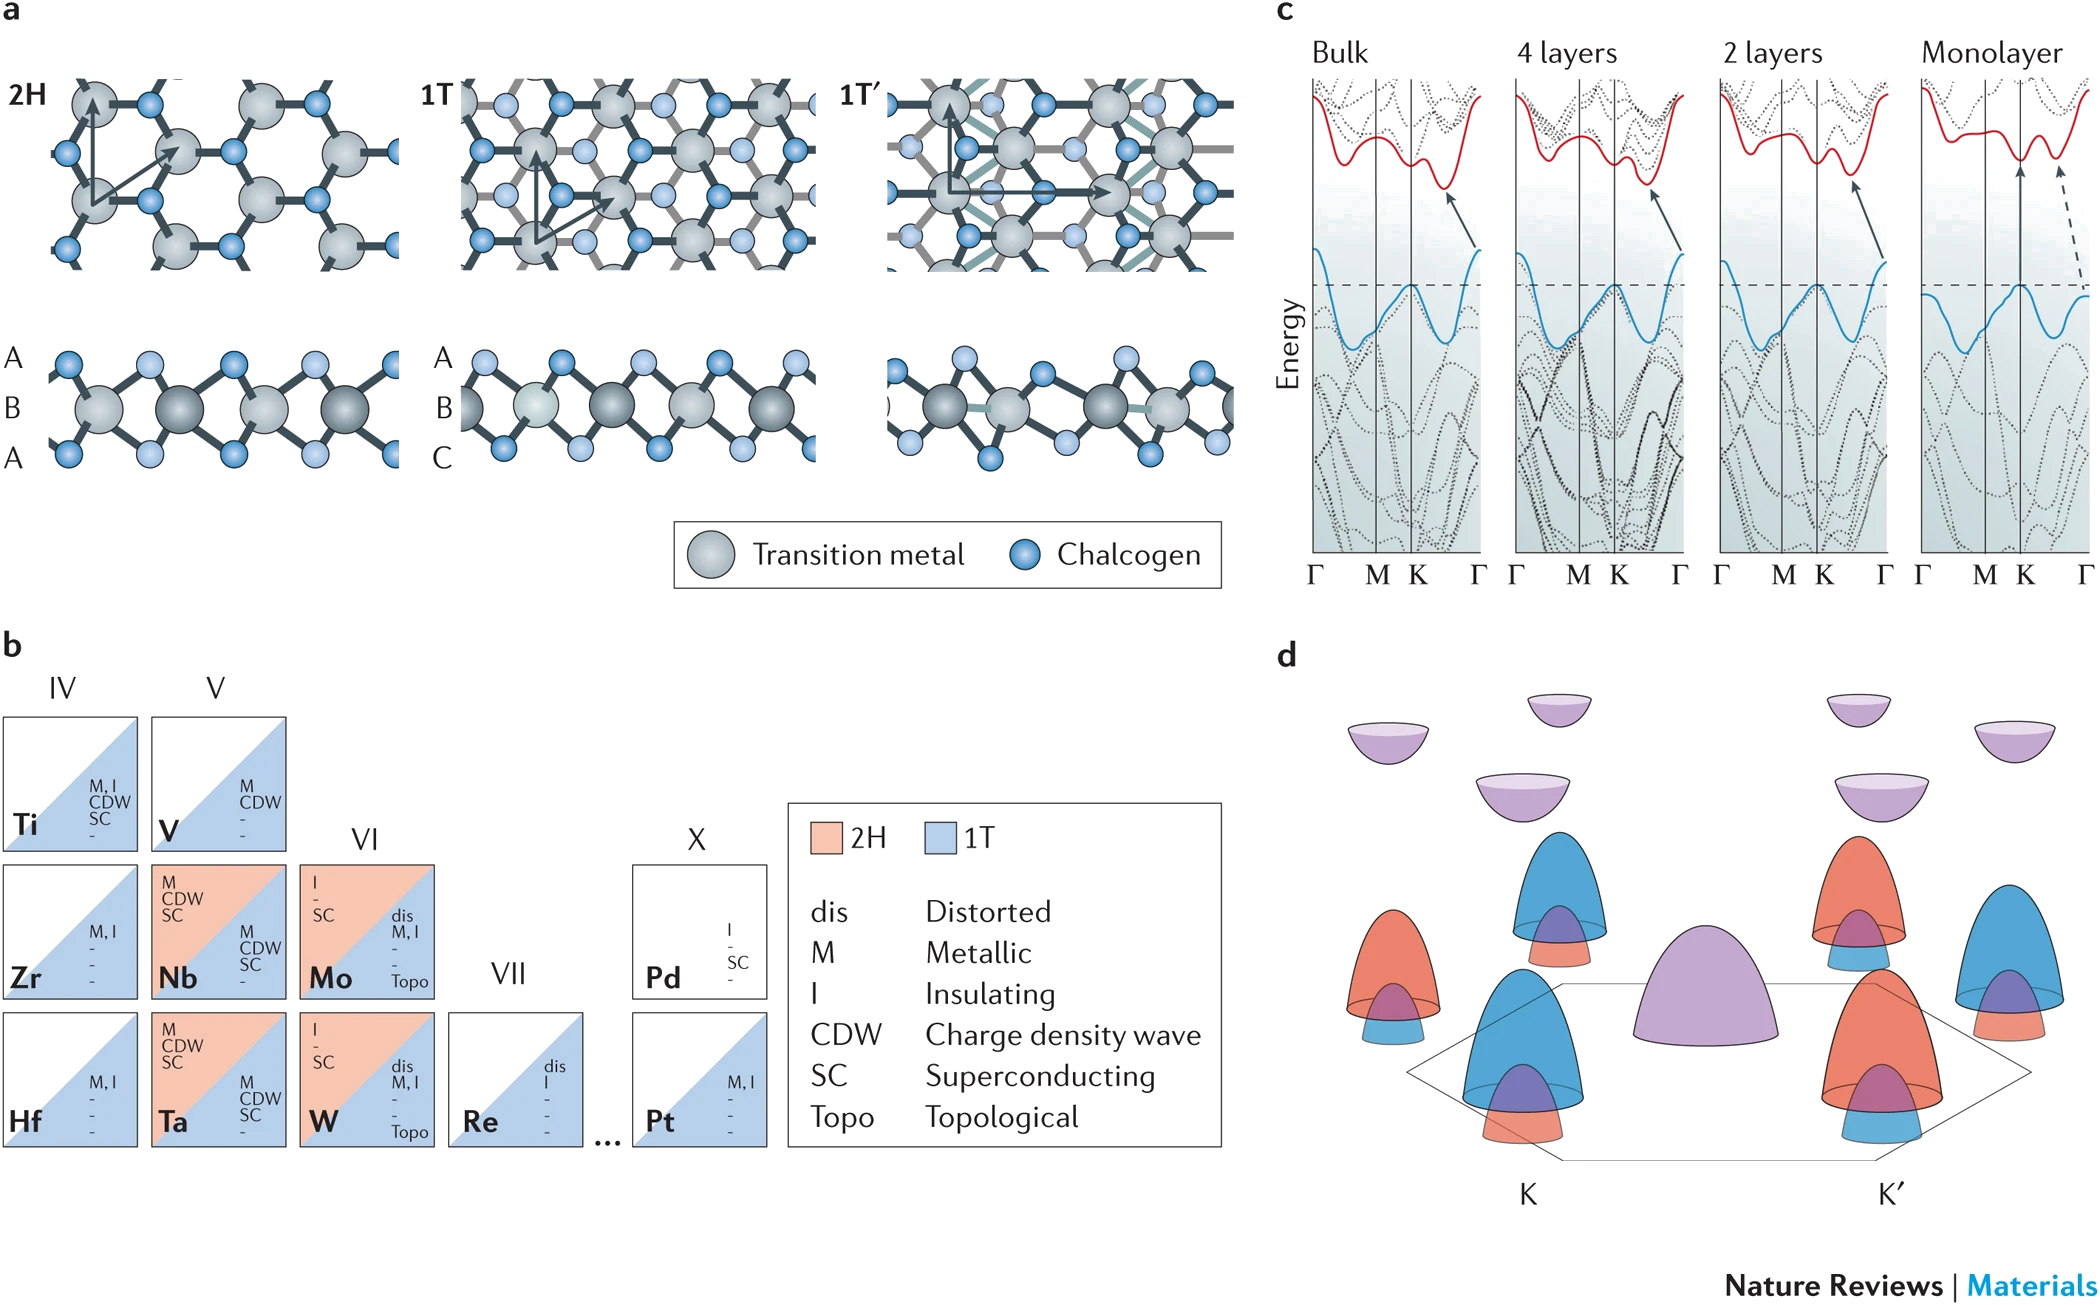
\includegraphics[width=1.0\textwidth]{figures/TMD.png}
    \caption{\textbf{Structure and electronic properties of TMDs} adapted from Ref. \cite{manzeli20172d}. \textbf{a |} Atomic structure of single layers of TMD in their \emph{trigonal prismatic} (2H), \emph{distorted octahedral} (1T) and \emph{dimerized} (1T') phases. \textbf{b |} ``Periodic table'' of known layered TMDs, organized based on the transition metal elements, their existing structural phases (2H, 1T and 1T'), and the observed electronic phases (see the right panel). \textbf{c |} Evolution of the band structure of 2H-MoS$_2$ from bulk material down to monolayers. Clearly a indirect gap to direct gap transition occurs for monolayer material only. \textbf{d |} Schematic band structure of 2H-MoS$_2$, showing the spin splitting (orange and blue colors) at K and K' points.)}
    \label{fig:TMD_electonic_properties}
\end{figure}
We will mostly focus on the group V and group VI transition metal elements, particularly those with 1T and 1T' phases shown to be unstable. So without loss of generalization, when we talk about monolayer TMDs in this thesis, we always refer to the 1H phase structure.
% \begin{figure}[!htp]
%     \centering
%     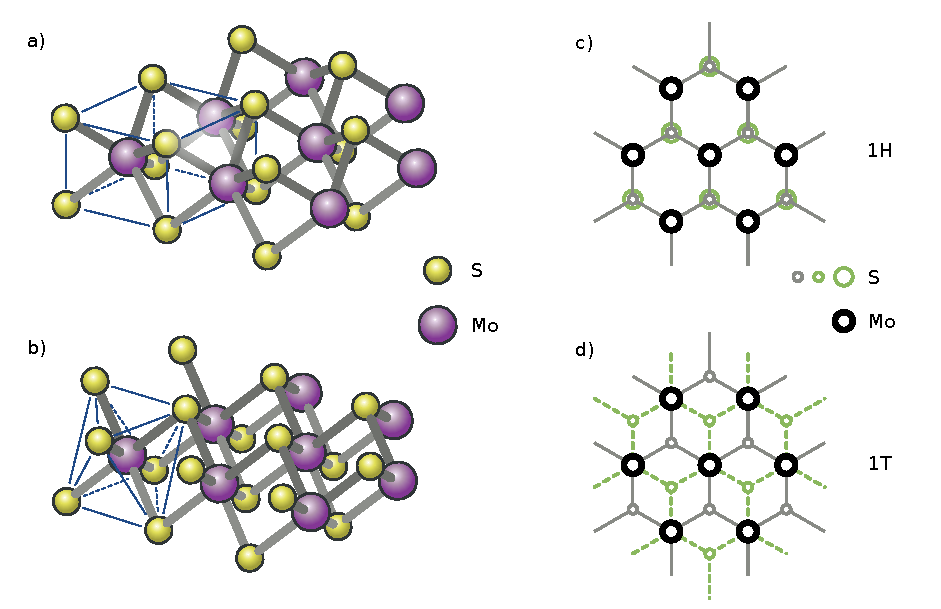
\includegraphics[width=0.8\textwidth]{figures/MoTe2_crystal_structure.pdf}
%     \caption{\textbf{Monolayer $\mathrm{MoS_2}$} (extracted from \url{https://en.wikipedia.org/wiki/Transition_metal_dichalcogenide_monolayers}). a) and c) for 1H phase of monolayer $\mathrm{MoS_2}$, and b) and d) for 1T phase of $\mathrm{MoS_2}$, which is \emph{metastable}. c) and d) are schematic top views, respectively. The 1H ground state has prismatic structure of chalcogen atoms surrounding the transition metal atoms, and the top/bottom layer of chalcogen atoms are the same. The metastable 1T phase shows octahedral structure, less relevant to our discussion, can be viewed by rotating all chalcogen atoms on the top layer by 30 degrees with respect to the lower layers.}
%     \label{fig:MoTe2_crystal_structure}
% \end{figure}
% The 1T phase is \emph{metastable} and is NOT relevant to our discussion. 


For monolayer TMDs of 1H phase, the corresponding bulk material are mostly of 2H stacking form, with alternating alignment of transition metal atoms and chalcogen atoms, as is shown in (a) in Fig. \ref{fig:MoS2_Di}.
\begin{figure}[!htp]
    \centering
    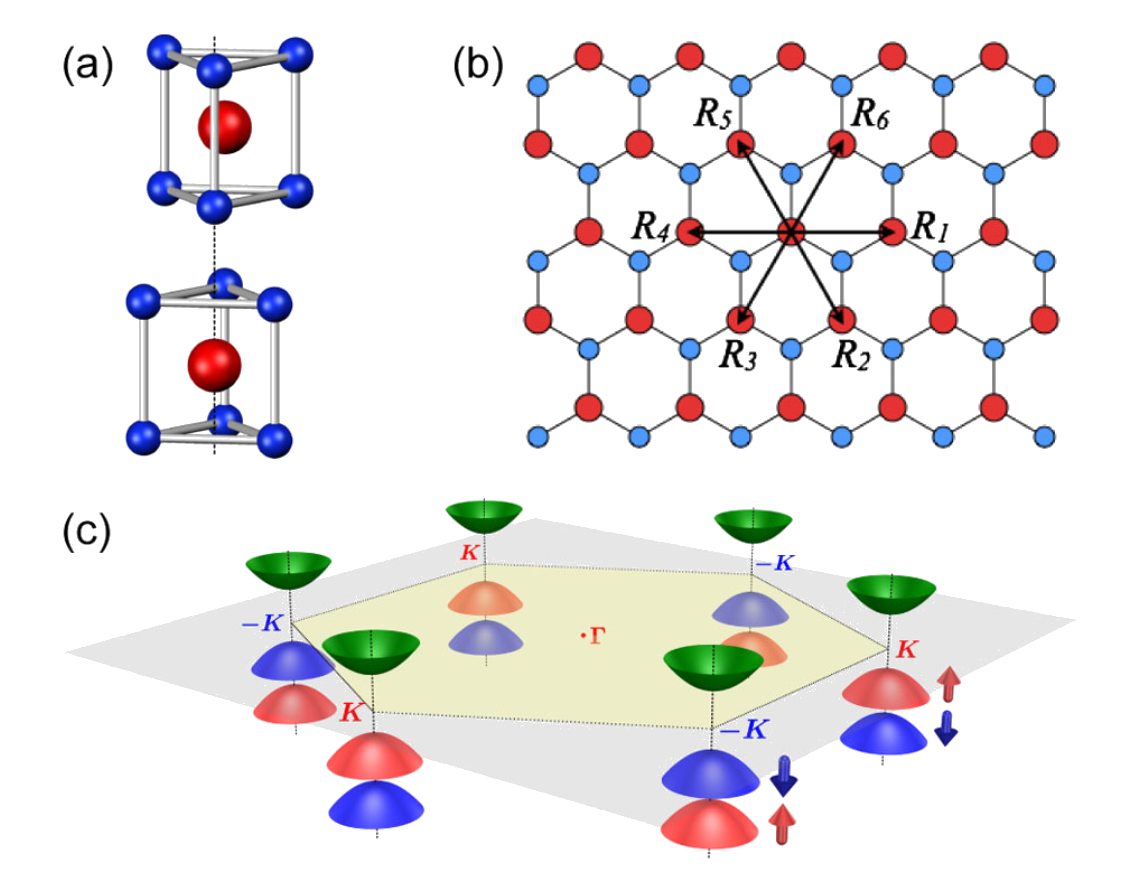
\includegraphics[width=0.8\textwidth]{figures/MoS2_Di.png}
    \caption{Figure adapted from Ref. \cite{xiao2012coupled}. (a) The unit cell of bulk 2H-MoS2. (b) Top view of MoS$_2$ monolayer. (c) Schematic drawing of the band structure at the band edges located at the K points.}
    \label{fig:MoS2_Di}
\end{figure}
Experimentally, there has been reports on the emergence of the peak in the optical spectroscopy study in Ref. \cite{mak2010atomically} and photoluminescence (PL) signals in Ref. \cite{splendiani2010emerging}, which is ascribed as the manifestation on the evolution of of the TMD band structure from bulk's indirect gap to monolayer's direct $K$-$K$ gaps, see (c) in Fig. \ref{fig:TMD_electonic_properties}.

Taking group-IV dichalcogenides MX$_2$ as the example, the 2H stacking bulk material has space group $D_{6h}$ with inversion symmetry (see (a) in Fig. \ref{fig:MoS2_Di}), but reduces to $D_{3h}$ breaking the inversion symmetry down to monolayers. For monolayer MX$_2$, DFT calculation tells that the relevant orbitals within the conduction and valence bands are all from partially-filled d-orbitals \cite{mattheiss1973band}. From symmetry aspect, the trigonal prismatic crystal field splits\footnote{See the character table for point group $D_{3h}$ \url{http://symmetry.jacobs-university.de/cgi-bin/group.cgi?group=603&option=4}.} the d-orbitals of transition metal elements into three groups: $A_1'(d_{z^2})$, $E'(d_{xy}, d_{x^2-y^2})$, and $E''(d_{xz}, d_{yz})$. But the in-plane $z\rightarrow-z$ mirror symmetry forbid the contribution from $E''$ (since both $d_{xz}$ and $d_{yz}$ changes sign under the mirror operation), leaving only $A_1'$ and $E'$ irreps contributing to the band structure.

Now we can start the $\bm k\cdot\bm p$ analysis around $K$ and $K'$ points. Clearly the only possibility to construct the two states orthogonal to each other (corresponding to $K$ and $K'$) is to insert the valley index $\tau=\pm1$ to the below irreps:
\begin{equation*}
    |\phi_1\rangle=|d_{z^2}\rangle, \quad|\phi_{2,\tau}\rangle=\dfrac{1}{\sqrt{2}}(|d_{xy}\rangle+i\tau|d_{x_2-y^2}\rangle)
\end{equation*}
And then the effective Hamiltonian can be expanded in terms of Pauli matrices as $H_\tau(\bm k)=\bm d(\bm k)\cdot\bm\sigma$. The diagonal parts represent the $K$-$K$ (or $K'$-$K'$) direct band gap $\Delta$. Up to the lowest order expansion, we can write
\begin{equation*}
    H=\begin{pmatrix}
        \Delta/2                 & \alpha k_x+\beta k_y \\
        \alpha^* k_x+\beta^* k_y & -\Delta/2
    \end{pmatrix}.
\end{equation*}
Then again due to $C_3$ symmetry, one can show that $\beta=i\alpha$ and we obtain the result
\begin{equation}\label{eq:MoS2 kdotp}
    H=\hbar v_F(\tau k_x\sigma_x+k_y\sigma_y)+\frac{\Delta}{2}\sigma_z.
\end{equation}

Now let us include the spin-orbit couplings (SOC) $\lambda\bm L\cdot\bm S$. This is equivalent to evaluate the matrix element $\langle \phi_{\alpha, s_1}|\bm L\cdot\bm S|\phi_{\beta, s_2}\rangle$.

\begin{equation}
    H_{\text{SOC}}=\lambda\bm\sigma\cdot(\nabla U\times\bm p)
\end{equation}

Standard $\bm k\cdot\bm p$ theory tells that the SOC contribution is to evaluate the

% \ref{fig:monolayer_TMD_band_structure}.
% \begin{figure}[!htp]
%     \centering
%     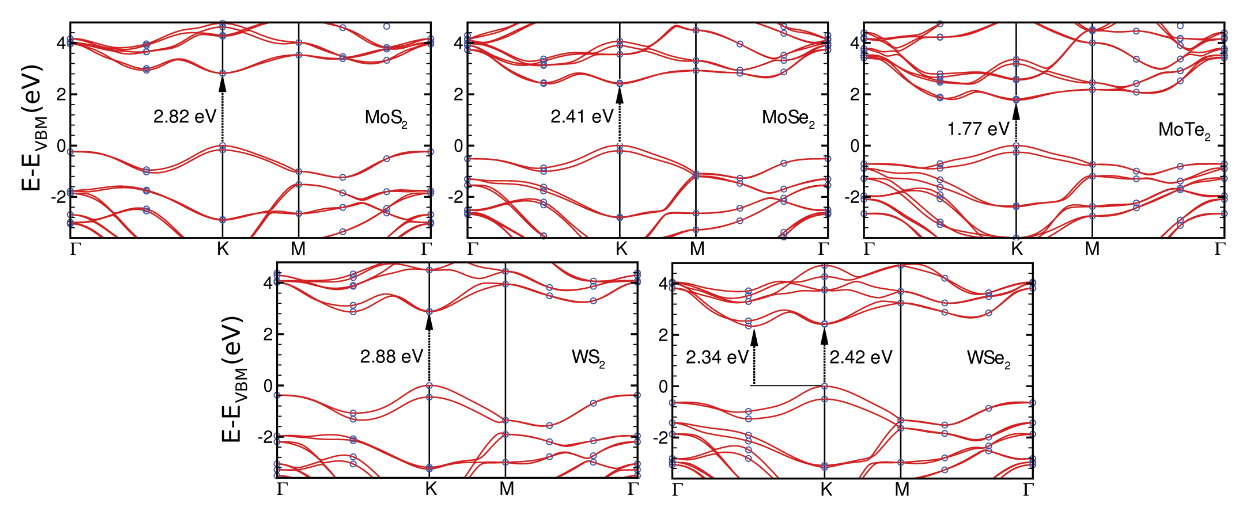
\includegraphics[width=0.8\textwidth]{figures/monolayer_TMD_band_structure.png}
%     \caption{DFT band structures for several MX$_2$ monolayer materials (extracted from \cite{ramasubramaniam2012large}).}
%     \label{fig:monolayer_TMD_band_structure}
% \end{figure}

% For typical monolayer TMD material, there are gap

% The M-X bonds within layers are mostly covalent, while weak Van der Waals forces hold the sandwiched layers. A

% Taking the prototypical group-VI dichalcogenide as the example, for example $\mathrm{MoS_2}$, a nice feature of



\subsection{Twisting with Moir\'{e} Physics}
Moir\'e patterns are known as the interference patterns generated when two or more periodic structures are overlaid. The interference pattern exhibits a new large-scale periodic structure (coin as \emph{Moir\'{e} scale}) on top of the original one, so that the original lattice information is smeared out, leaving physics occurring at such new Moir\'{e} scale $a_M\sim a/\theta$. In momentum-space, this is equivalent to have a largely reduced Moir\'e Brillouin zone (mBZ) with the Moir\'e reciprocal vector $b_M\sim \theta b$, \textbf{giving rise to a large number of $N_M\sim N/\theta^2$ Moir\'e bands due to the \emph{zone folding effect}}. This is desirable since the new Moir\'e unit cell now encloses a number of $N_M\sim N/\theta^2$ atoms from the $N$ atoms within the orignal unit cell. Clearly not all value of $\theta$ gives an integer $N_M$. Those $\theta$ that indeed gives an integer $N_M$ are \emph{commensurate} angles. However, in the small twisting regime where $N_M\gg1$, it is OK to always take $N_M$ as an integer, and consider \emph{incommensurate angles} as well.

As a result, the band width $\Delta$ of the original periodic structure is also highly suppressed to $\Delta\theta^2$ within mBZ. Plus the possible tunnelings between different mBZ sectors, which has no reason to stay to be zero, we will naturally end up with gapped Moir\'e bands as isolated \emph{flat bands}, where strong correlations play important roles because the electron kinetics are almost quenched. To sum up, the Moir\'e Hamiltonian can be constructed as the following two steps:
\begin{enumerate}
    \item Enlarge unit cell to Moir\'e super unit cell, which is equivalent to partition the original BZ into many mBZ connected with Moir\'e reciprocal vectors. This serve as the diagonal part of the huge Moir\'e Hamiltonian.
    \item These mBZs can talk to each other through the interlayer tunnelings. This will serve as the off-diagonal part of the Moir\'e Hamiltonian.
\end{enumerate}

\subsubsection{Twisted Bilayer Graphene}
Before dive into the details, let us first fix the geometry of twisted bilayer graphene (tBLG). For each layer, we take the bravias vector $\bm a_1=\frac{a}{2}(\sqrt{3},3), \bm a_2=\frac{a}{2}(-\sqrt{3},3)$ with the sublattice crystal vector $\bm\delta_A=\bm 0, \bm\delta_B=\frac{1}{3}(\bm a_1+\bm a_2)$, so that the reciprocal vector reads $\bm b_1=\frac{2\pi}{3a}(\sqrt{3},1), \bm b_2=\frac{2\pi}{3a}(-\sqrt{3},1)$, and the BZ edge $K$-point is $\bm K=\frac{1}{3}(\bm b_1-\bm b_2)$. Monolayer graphene is known for the presence of Dirac points at $K$ (or $K'$) points. Denoting the layer index as $l=\pm1$, we can start with stacking two Dirac cone Hamiltonian around $K$ (or $K'$) point with separated top/bottom bloch basis ${|\bm k_l,\alpha\rangle}$
\begin{equation*}
    H_K = \sum_{l=\pm 1}\sum_{\bm k_l\in\text{BZ}_l}\sum_{\alpha\alpha'} c_{\bm k_l,\alpha'}^\dagger \hbar v_F[(\bm k_l-\bm K_l)\cdot\bm\sigma]_{\alpha'\alpha} c_{\bm k_l,\alpha}.
\end{equation*}

As is discussed above, if we stack two layers of graphene with a relative commensurate twist angle $\theta$. The Moir\'e Hamiltonian should be constructed by partitioning the sum of orignal Bloch states $|\bm k\rangle$ for $\bm k\in\text{BZ}$ into the sum within the mBZ, plus the sum over distinct mBZ sectors connected with Moir\'e reciprocal vectors
\begin{equation*}
    \{|\bm k_l\rangle\}_{\bm k_l\in\text{BZ}}\rightarrow\{|\bm k_l+\bm Q_l\rangle\}_{\bm k_l\in\text{mBZ},\bm Q_l=\{l_1\bm b_{M1}+l_2\bm b_{M2}\}}.
\end{equation*}

As is seen in Fig. \ref{fig:tBLG_geometry}.

\begin{figure}[!htp]
    \centering
    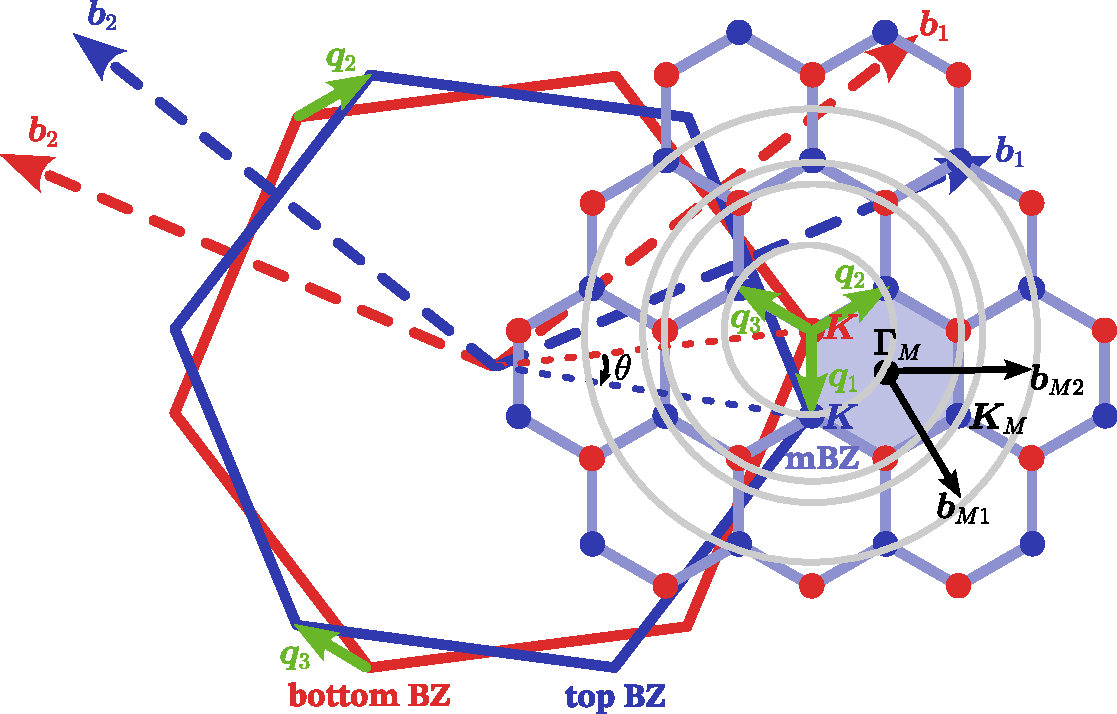
\includegraphics[width=0.95\textwidth]{figures/tBLG_geometry.pdf}
    \caption{Moir\'e Brillouin Zone of Twisted Bilayer Graphene. Blue (top) hexagonal BZ is rotated by $-\theta/2$, red (bottom) hexagonal BZ is rotated by $\theta/2$. The Moir\'e BZ (mBZ) is the shaded hexagonal. Gray dashed circles represents the truncation shells for the interference of interlayer tunnelings.}
    \label{fig:tBLG_geometry}
\end{figure}

Next step is to consider the tunnelings among each mBZ sectors. Generally, this is to think about the interlayer tunneling matrix elements for some interlayer tunneling Hamiltonian $H_{\text{interlayer}}$:
\begin{align*}
    T_{\bm k_l,\alpha;\bm k_{l'},\alpha'} & = \langle\bm k_l,\alpha|H_{\text{interlayer}}|\bm k_{l'},\alpha'\rangle                                                                                                                                                                 \\
                                          & \equiv\frac{1}{N}\sum_{\bm R_l,\bm R_l'}\sum_{\alpha,\alpha'} e^{-i\bm k_l\cdot(\bm R_l+\bm\delta_{l,\alpha})}e^{i\bm k_{l'}\cdot(\bm R_{l'}+\bm\delta_{l',\alpha'})}t(\bm R_l+\bm\delta_{l,\alpha}, \bm R_{l'}+\bm\delta_{l',\alpha'})
\end{align*}
where we recognize the real-space tunneling between Wannier centers $\langle\bm R_l,\alpha|H_{\text{interlayer}}|\bm R_l',\alpha'\rangle\equiv T(\bm R_l+\bm\delta_{l,\alpha}, \bm R_{l'}+\bm\delta_{l',\alpha'})$. And because Wannier center is highly localized, \emph{two-center approximation} \cite{bistritzer2011moire} can be made so that $T(\bm R_l+\bm\delta_{l,\alpha}, \bm R_{l'}+\bm\delta_{l',\alpha'})\simeq T(\bm R_l+\bm\delta_{l,\alpha} - \bm R_{l'}-\bm\delta_{l',\alpha'})$. Introducing the Fourier component of the the real-space tunneling $t_{ll'}^{\alpha\alpha'}(\bm q)$ (due to translation symmetry)
\begin{align*}
    T(\bm R_l+\bm\delta_{l,\alpha} - \bm R_{l'}-\bm\delta_{l',\alpha'}) & = \frac{1}{N}\frac{1}{A}\sum_{\bm q}t_{ll'}^{\alpha\alpha'}(\bm q) e^{i\bm q\cdot(\bm R_l+\bm\delta_{l,\alpha} - \bm R_{l'}-\bm\delta_{l',\alpha'})},
\end{align*}
we have
\begin{align}
    T_{\bm k_l,\alpha;\bm k_{l'},\alpha'} & =\frac{1}{A}\sum_{\bm q}\left(\frac{1}{N}\sum_{\bm R}e^{i\bm R_l\cdot(\bm q-\bm k_l)}\right)\left(\frac{1}{N}\sum_{\bm R'}e^{-i\bm R_{l'}\cdot(\bm q-\bm k_{l'})}\right) \sum_{\alpha\alpha'} t_{ll'}^{\alpha\alpha'}(\bm q) e^{i\bm \delta_{l,\alpha}\cdot\bm(\bm q-\bm k_l)}e^{-i\bm\delta_{l',\alpha'}\cdot(\bm q-\bm k_{l'})} \nonumber \\
                                          & = \frac{1}{A}\sum_{\bm q}\sum_{\bm G_l}\delta_{\bm q-\bm k_l,\bm G_l}\sum_{\bm G_{l'}}\delta_{\bm q-\bm k_{l'},\bm G_{l'}}\sum_{\alpha\alpha'} t_{ll'}^{\alpha\alpha'}(\bm q) e^{i\bm \delta_{l,\alpha}\cdot\bm(\bm q-\bm k_l)}e^{-i\bm\delta_{l',\alpha'}\cdot(\bm q-\bm k_{l'})}                                                \nonumber \\
                                          & = \sum_{\bm G_l,\bm G_{l'}}\sum_{\alpha\alpha'} \frac{t_{ll'}^{\alpha\alpha'}(\bm k_l+\bm G_l)}{A} e^{i\bm\delta_{l,\alpha}\cdot\bm G_l}e^{-i\bm \delta_{l',\alpha'}\cdot\bm G_{l'}}\delta_{\bm k_l+\bm G_l,\bm k_{l'}+\bm G_{l'}}.\label{eq:two-center_approximation}
\end{align}
The momentum-space expression Eq. \eqref{eq:two-center_approximation} is the general result of the two-center approximation. The Dirac delta function signatures the momentum convervation of the tunneling processes.

In the setup of twisted bilayer graphene, Eq. \eqref{eq:two-center_approximation} can be further simplified by looking at the small shift around the $K$ or $K'$ point $\bm k_l\rightarrow\bm k_l+\bm K_l$ for $|\bm k_l|\ll1$.



\subsubsection{Twisted TMD}
For bilayer Moir\'e materials, the Moir\'e interference patterns can be formed when two layers (not have be fully identical) are relatively displaced with a vector $\bm d$ and properly rotated by some \emph{commensurate} angle $\theta$.


It has been already shown in monolayer group-IV TMDs that the strong spin-orbit coupling and broken inversion symmetry lifts spin degeneracy within the conduction band $\sim100$meV. Thus for a bilayer TMD material of the same kinds (\emph{homobilayer}), for example, twisted bilayer MoTe$_2$, the $K$ or $K'$ valley valence band (pinned with spin) can be separated out in our discussion, resulting a simple two-band model with layer pseudospin at each valley.



\subsection{Twisting without Moir\'{e} Physics}
\subsubsection{Twisted Cuprates}
